\subsection{Positive Selection Inference}
\label{sec:selection-inference}

This section presents the proposed mechanism for gene selection inference and design of validation experiments performed to test it.

\begin{sidewaysfigure}
  \centering
  \begin{minipage}{.7\textwidth} % adjust the width as needed

    \begin{minipage}{\textwidth}
      \centering
      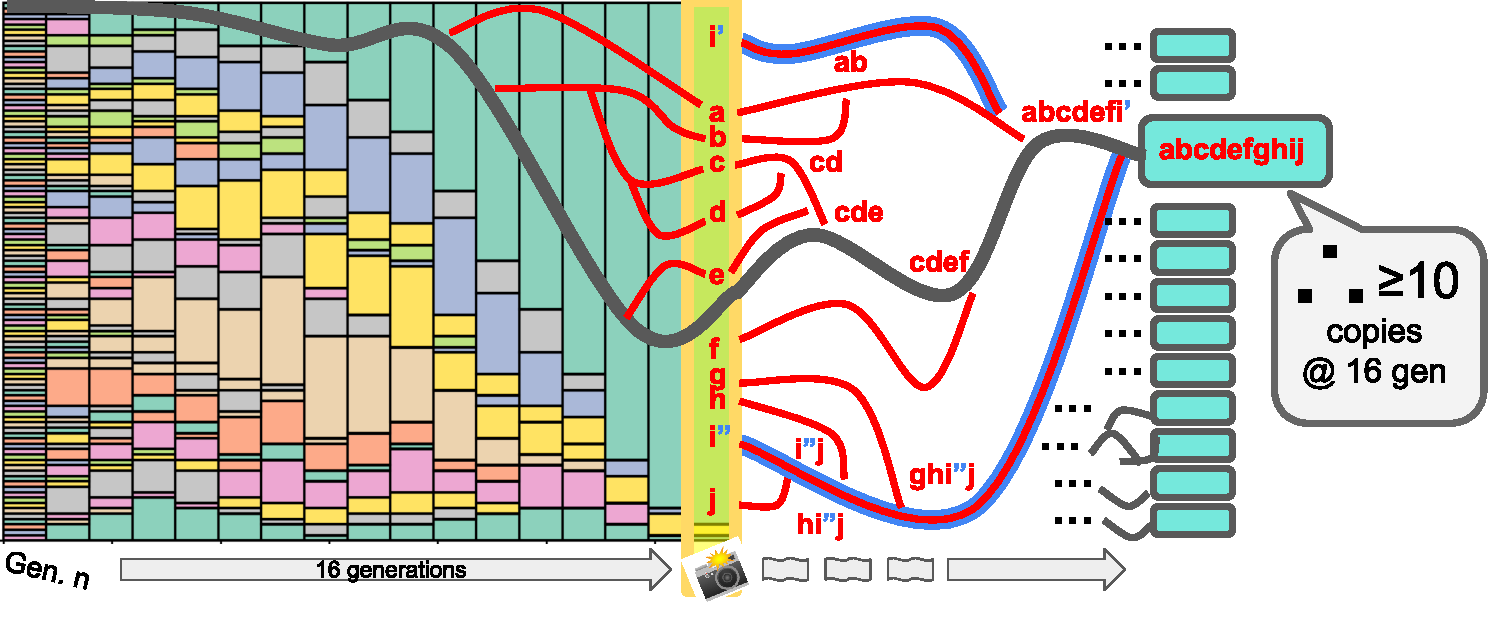
\includegraphics[height=0.30\textheight]{img/copy-count-snapshot}
      \subcaption{Cartoon depiction of delayed copy count estimation mechanism, annotated over Muller plot depicting weak selection over focal allele.
      }
      % \label{fig:ne-example-replicates:bottleneck}
    \end{minipage}%

    \vspace{1cm}

    \begin{minipage}{0.5\textwidth}
      \centering
      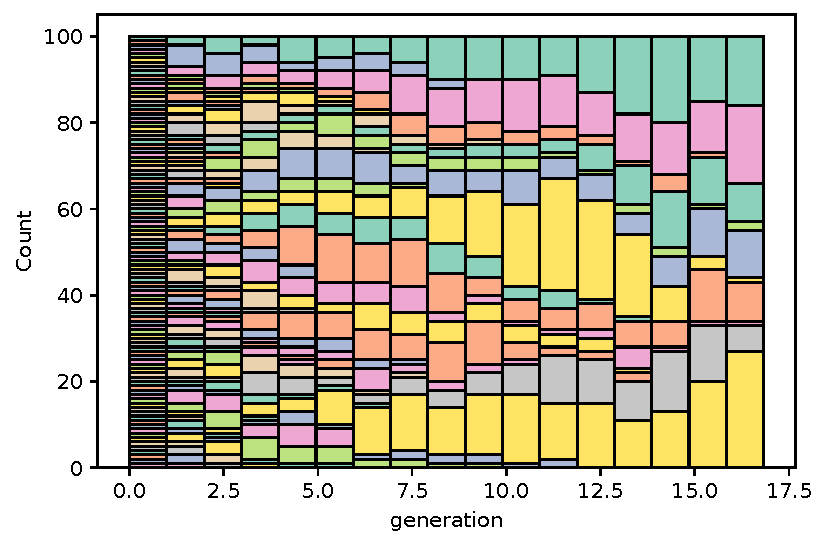
\includegraphics[height=0.2\textheight]{notebooks/notebooks/teeplots/fit=0.0+hue=clade+multiple=stack+ngen=16+npop=100+palette=set2+viz=histplot+x=generation+ext=}
      \subcaption{Muller plot depicting no selection for focal allele, ending with smaller copy count after 16 generations.}
      % \label{fig:ne-example-replicates:selection_pressure}
    \end{minipage}%
    \begin{minipage}{0.5\textwidth}
      \centering
      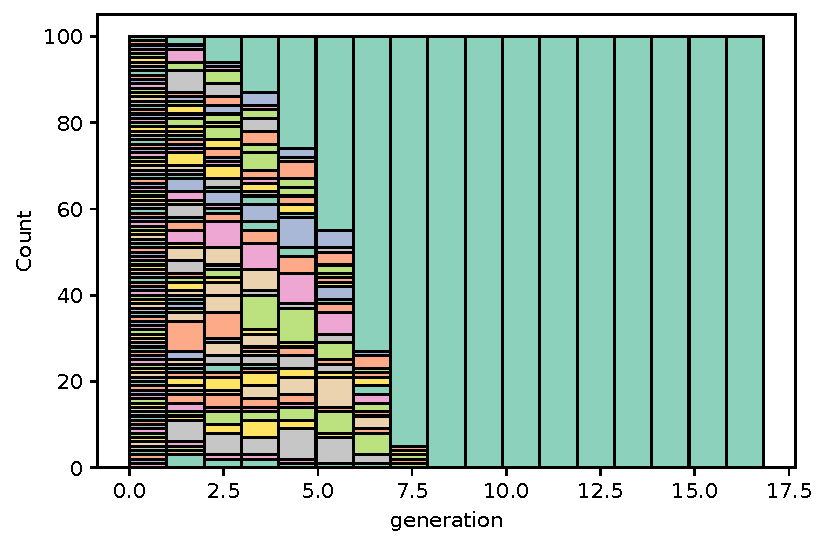
\includegraphics[height=0.2\textheight]{notebooks/notebooks/teeplots/fit=1.0+hue=clade+multiple=stack+ngen=16+npop=100+palette=set2+viz=histplot+x=generation+ext=}
      \subcaption{Muller plot depicting strong selection for focal allele, with fixation occuring before 16 generations.}
      % \label{fig:ne-example-replicates:control}
    \end{minipage}

  \end{minipage}
  \hfill % Creates horizontal space. Can also use \hspace{<len>}
  \begin{minipage}{.25\textwidth} % adjust the width as needed
    \caption{
      Proposed mechanism for detecting gene-level selection via a distributed delayed copy count estimation mechanism.
      Strata deposited at generation $n$ progress through 16 generations, with copy count of one allele growing due to selection.
      On the sixteenth generation, a ``snapshot'' is performed to set a random bit on field annotated onto each descendant differentia copy.
      In subsequent recombination events, set bits are exchanged between bit fields associated with common differentia.
      Copy count at generation $n + 16$ from can then estimated from these bit fields, with high copy count being suggestive of selection.
      Note that in this example collision between set bits $i'$ and $i"$ result in an undercount.
      This mechanism is associated with ``gene-level'' instrumentation (Figure \ref{fig:annotation-types}).
    }
    \label{fig:ne-example-replicates}
  \end{minipage}

\end{sidewaysfigure}


% notebooks/notebooks/teeplots/notebook=ne-inference+replicate=0+treatment=bottleneck+viz=plot-running-estimation+x=rank+y=population-size+ext=.pdf
%
% notebooks/notebooks/teeplots/notebook=ne-inference+replicate=0+treatment=control+viz=plot-running-estimation+x=rank+y=population-size+ext=.pdf
%
% notebooks/notebooks/teeplots/notebook=ne-inference+replicate=0+treatment=range-expansion+viz=plot-running-estimation+x=rank+y=population-size+ext=.pdf
%
% notebooks/notebooks/teeplots/notebook=ne-inference+replicate=0+treatment=selection-pressure+viz=plot-running-estimation+x=rank+y=population-size+ext=.pdf

\textbf{Inference Mechanism.}
Increases in allele prevalence tend to occur for alleles experiencing positive selection, but can also occur for selectively neutral alleles due to drift effects.
The key difference between the two is the \textit{rate} of increase within the population --- increases in prevalence due to drift tend to be slower than increases in prevalence due to selective effects, especially for large population sizes.

The proposed instrumentation mechanism uses gene-wise hereditary stratigraph instrumentation.
Selection is differentiated from drift dynamics by capturing an estimate of copy count of each gene's descendants after a fixed number of generations $g$ elapse.
If this copy count falls in the tails of the distribution expected after $g$ generations under a null hypothesis of pure drift dynamics, positive selection can be inferred.
Stronger positive selection will correlate with more extreme changes in copy count within the $g$ generation window.

In order to record estimated copy count, each ``fingerprint'' differentia within genes' hereditary stratigraph is bundled with an additional fixed-length, zero-initialized bit field annotation upon creation.
Each ``fingerprint'' has its own associated supplementary annotation.
This bit field is copied verbatim to descendants (i.e., gene copies passed to organismal offspring).

When the $g$th generation following a ``fingerprint'' differentia's creation elapses, a single bit is set at a random position of the supplementary annotation bit field.
During crossover, bit field annotations from the same generation with matching differentia are or'ed bitwise with each other.
In this manner, set bits gradually propagate among the records of all gene copies maintained in the population.

In this manner, annotations' bit counts converge to reflect the number of gene copies present after generational delay $g$.
Figure \ref{fig:copy-count-snapshot} summarizes the entire proposed distributed delayed copy count estimation mechanism.
Under count of gene copies is possible under this mechanism (due to positional collisions between set bits or gene copy extinctions immediately subsequent to generation $g$), but --- notably --- over count is not.
This conservative property supports confident detection of selection events --- these events would only be falsely detected due to true increases in copy count through drift, not due to instrumentation-associated error.%
\footnote{This conservative property holds under the assumption of no spurious differentia collision.}
(This said, this conservative property could be sacrificed to increase sensitivity to larger copy counts with a given width bit field by only setting a bit at generation $g$ with small probability $p$.)

A bit field with of 8 bytes and a snapshot delay of 16 generations were arbitrarily chosen for experiments reported here.
Better sensitivity to weak selection events should be achievable through longer snapshot windows and larger bit fields, but likely this will be at the cost of diluting signal from strong selection events.
Future work should seek a principled procedure to decide appropriate snapshot window length and bit field widths apropos of experimental objectives and properties of the underlying evolutionary system (i.e., selection pressure).

Positive selection can occur without advent of new allelic variants --- changes in environmental conditions can induce positive selection on an existing, potentially widespread allelic variant that was previously neutral.
This scenario is called a ``soft'' sweep \citep{hermisson2005soft}.
Soft sweeps should, in principle, be detectable to some extent through this methodology, as they involve increases in copy count at faster-than-drift rates.
However, weak sweeps on very-widespread alleles that quickly reach fixation will register only a weak signal on this instrumentation because increases in descendant copy count are spread across the large number of preexisting allele copies.
Although detectability of weak sweeps are not tested in this work, this issue merits consideration in future work.

\textbf{Validation Experiment.}
A minimalistic experimental system was devised to test proposed methodology to detect positive selection on a novel allele.
We model the introduction of an atomic gene with tunable fitness advantage into an otherwise neutral background.

Each individual in the population was represented by a single floating-point number, representing a single focal gene.
Gene values were restricted between 0.0 and 1.0.
Fitness score was defined as the sum of its own value and a random number drawn from a continuous, uniform unit-valued distribution.
So, individuals' gene value corresponded directly to probabilistic fitness advantage.
For example, a value of 0.2 would give an average 20\% selective advantage.
Fitness scores for each individual were calculated once per generation and used for all tournaments.

All individuals were initialized with gene value 0.0.
At generation 50, one organism's gene value was set to either 0.0,\footnote{The smallest representable floating point value was set for fitness advantage treatment 0.0 so the introduced gene could be differentiated from the background gene.
This value was small enough as to have no meaningfully detectable effect on selection.} 0.1, or 1.0.
This operation was repeated at subsequent generations if the introduced gene value went extinct.
This procedure enabled comparison of a strong selective sweep for the gene (fitness advantage 1.0), a weaker selective sweep for the gene (fitness advantage 0.1) and a control treatment where no fitness advantage was introduced and pure drift dynamics were at play (fitness advantage 0.0).
Underlying selective sweep dynamics were measured by recording gene copy count at each generation.

Synchronous selection with tournament size 2 was performed each generation.
200 generations were simulated, with a constant population size of 400.
All parents for the upcoming population were selected before turnover of the entire population.
The crossover mating operator selected a gene value from among the two parents' genes with equal probability.
No mutation was applied.
Ten independent replicates were performed of each treatment.
